\documentclass[a4paper, 12pt]{ctexart}
\usepackage{amsfonts}
\usepackage{amsmath}
\usepackage{graphicx}
\usepackage{indentfirst}
\usepackage{pythonhighlight}

\usepackage[colorlinks, citecolor=red]{hyperref}

\usepackage{array}
\usepackage{multirow}
\usepackage{fullpage} % Set margins and place page numbers at bottom center
%\usepackage{fancyhdr}    
%\usepackage{lastpage}
%\pagestyle{fancy} %fancyhdr宏包%新增的页面风栌
%\fancyhf{}
%
%\cfoot{Page \thepage\ of \pageref{LastPage}}%圓前页  of 总页数
% == 代码倄理
\usepackage{listings}
\lstset{
    columns=flexible,
    breakatwhitespace=false,
    breaklines=true,
    frame=single,
    numbers=left,
    numbersep=5pt,
    showspaces=false,
    showstringspaces=false,
    showtabs=false,
    stepnumber=1,
    rulecolor=\color{black},
    tabsize=2,
    texcl=true,
    escapeinside={\%*}{*)},
    extendedchars=false,
    mathescape=true,
}

\setlength{\evensidemargin}{-0.05in}
\setlength{\oddsidemargin}{-0.05in}
\setlength{\headheight}{-0.2in}
\setlength{\headsep}{0in}
\setlength{\textheight}{9.75in}
\setlength{\textwidth}{6.5in}


\renewcommand{\baselinestretch}{1.5}
% == 汉化
\renewcommand{\figurename}{图}
\renewcommand{\tablename}{表}

\begin{document}

\title{基于MemoryNetwork的推特流行度预测}
\author{盛俊杰,徐洪义,黄金根}
\date{10152510150,etc}
\maketitle
%\thispagestyle{fancy}


% ————————
\section{问题描述}
这次大作业我们小组选择的是推特流行度预测问题,通过用户之前发出的推特的内容,标签,转载数,以及用户自身的follower\_cnt和statuses\_cnt来预测一条新发的推特的最终转载数。
% ————————
\section{数据分析}
我们所获得数据如下

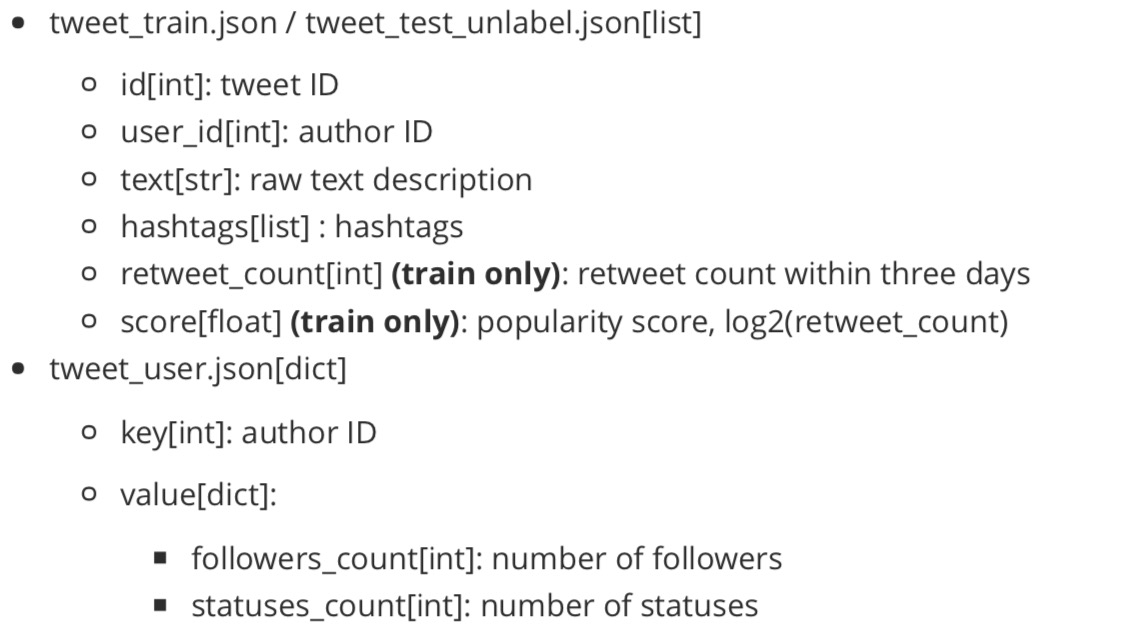
\includegraphics[width=6inc]{tweet_pics/data}

需要预测的任务是

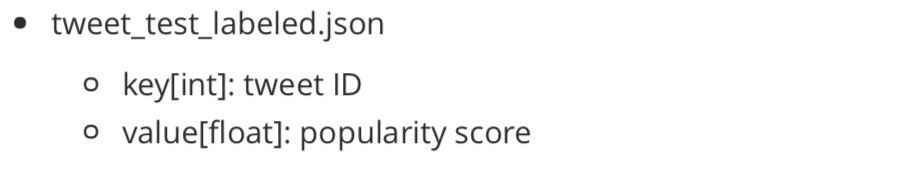
\includegraphics[width=6inc]{tweet_pics/task}

可以看到我们需要预测的是一条tweet的$ popularity score$ ,而可以用来建立模型的属性有$userid$,$text$,$hash\_tags$以及用户的特征$followers\_count$,$statuses\_count$。大致先看下各个属性的特征好了:
\begin{enumerate}
	\item $text$:文本数据,包含特殊字符(需要去除),长度一般在60words以内
	\item $userid$:用户id,训练集中有总共134个用户
	\item $hash\_tags$:标签,有413个标签
	\item $followers\_count$:关注者数目50W~3500W之间
	\item $statuses\_count$:发布状态数1W~165W之间
\end{enumerate}

再来看一下$retweet\_count$的分布:

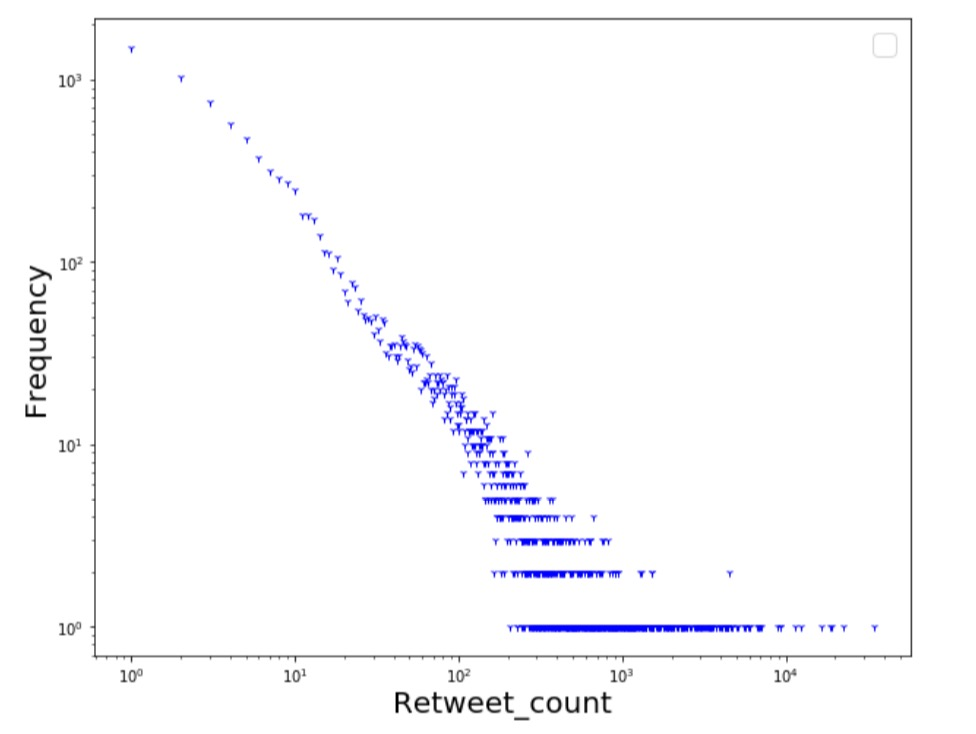
\includegraphics[width=6inc]{tweet_pics/0}

可以看出高转发数的tweet出现频度是很低的,而大部分的转发数都是维持在较低的水平。

\section{模型阐明}
在这里我们采用的方法是使用Memory NetWork与张量分解结合形成的一个端到端的模型,原文中称之为MOOD模型。使用Memory NetWork获得文本的最佳表示,
\subsection{模型总览}
整个模型的输入由$userid$,$text$,$hash\_tags$,$followers\_count$,$statuses\_count$组成,核心可分为Memory Network与Tensor Factorization两部分。模型图见下

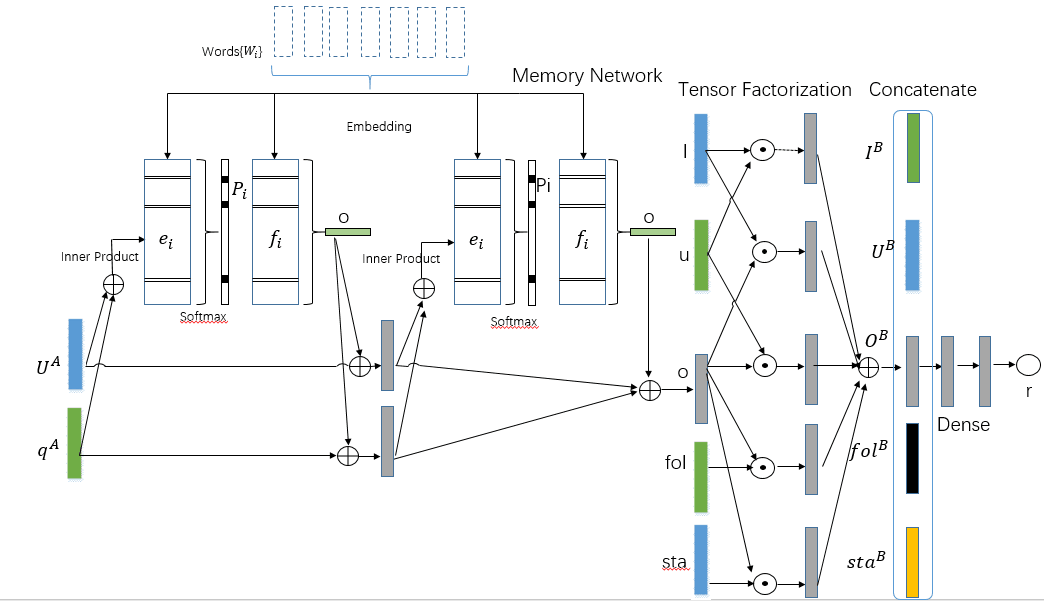
\includegraphics[width=6inc]{tweet_pics/model}
\subsection{Memory Network}
\subsubsection{Memory Representation}
在这个模块中,MOOD分别定义了memories for word,user和hash\_tag。我们设字典大小为$|V|$,文档长度为$L$,嵌入维度为k(这里又进一步假设userid,hash\_tag的嵌入维度也为k),我们将每一个单词都与user和hash\_tag相关联,同时又为了考虑词序信息,我们将两个绝对位置编码矩阵$E^p \in \mathbb{R}^{k\times L}$和$F^p \in \mathbb{R}^{k \times L}$合并到基本词嵌入中。
同时,MOOD定义user和hash\_tag的注意嵌入矩阵$U^A \in \mathbb{R}^{k\times\left| Q \right|}$。那么有$u_u^A=U_{:,u}^A$和$q_q^A=Q_{:,u}^A$
\subsubsection{Attention for Memory}
在原始词汇空间中,文本介绍可以表示为一个热编码的序列(虽然在实现时我们是直接记录词典索引序列的,但为了论文描述方便).对于引言d中的第j个单词$w_j$,热编码向量表示为$\hat{w_j} \in \left\{  0,1\right\}^ {\left| V \right|} $。假设$v(j)$示词汇表中$w_j$的索引,我们可以得到嵌入$e_{v(j)}=E\hat{w_j}+E_{:,j}^p$以类似的方式,也可以获得$f_{v(j)}$

基于这些嵌入,MOOD通过以下等式计算关于v(j)的user u和hash\_tag q的关注权重:
\[w_{v(j)}^{u,q}=(u_u^A+q_q^A)^Te_{v(j)}\]
这样我们就同时考虑进去了user和hash\_tag两个特征。
\subsubsection{Output Representation of Text}
内存网络模块的核心目标是获得更好的活动介绍表示。首先计算$p_{v(j)}^{u,q}=softmax(w_{v(j)}^{u,q})$代表v(j)表示d的重要性的概率。单层记忆网络中学习到的d的表示记为o:
\[o= \sum_{j}p_{v(j)}^{u,q}f_{v(j)}\]
\subsubsection{Multi-layered Extension}
类似于深度记忆网络采用的共同策略,MOOD更新了每层之间的组织者和位置嵌入。Organizer u和location q在第k层的嵌入分别表示为$u_u^{A,K}$和$q_q^{A,k}$。对于第一层,有$u_u^{A,1}=u_u^A$和$q_q^{A,1} = q_q^{A}$.按如下公式化迭代更新:
\[u_u^{A,K+1}=u_u^{A,K}+o^k\]
\[q_q^{A,K+1}=q_q^{A,K}+o^k\]

\subsection{Tensor Factorization}
在张量分解模块中,MOOD定义了$userid$,$text$,$hash\_tags$,$followers\_count$,$statuses\_count$的交互嵌入。它将五种嵌入模型组合在一起,以捕捉它们对活动流行度的共同影响。这个交互嵌入其实可以有怪多种定义方式,这里使用简单的乘积求和表达。公式如下:
\[\psi_d^{u,q}=u_u^{I} \bigodot q_q^{I}+u_u^{I} \bigodot o_d+q_q^{I} \bigodot o_d+f_f^{I} \bigodot o_o^{I}+s_s^{I} \bigodot o_o^{I}\]

通过经验可知(玄学),$userid$,$hash\_tags$,对于评分还是有很明显的偏置作用的。于是引入用户u和标签q的偏置嵌入$u_u^B$和$q_q^{B}$
我们进一步连接偏置嵌入和集成嵌入,并将它们与完全连接层相关联以计算流行度$\hat{r}$:
\[\hat{r}=\Theta^T\sigma(W_1^T[\psi_d^{u,q};u_u^B;q_q^B]+b_1)+b\]

这里我们对其进行了改进,考虑到部分user在训练集出现次数较低,我们可能无法通过那少量的数据习得用户的特征,所以在concate时我们加入$followers\_count$,$statuses\_count$两层,来更好的更话用户特征对流行度的预测。而在全连接层上我们选择了2层的隐层(全连接),再全连接到节点数为1的输出层。

\section{代码构建}
\subsection{预处理}
首先我们对text进行处理,首先进行预处理,去除链接与特殊字符,再进行词典编码,为了保留词序信息,这里我们按顺序记录每个词语的index。实现如下

\begin{python}
# judge if containAlpha
def containAlpha(wo内存表示:在这个模块中,MOOD分别定义了单词,管理器和位置的内存rd):   
    if len(word) == 0:  
        return False
    else:  
        if re.search('[a-z]', word):  
            return True  
        else:  
            return False
# delete uri info
def deleteUri(text):
	textlist=text.split()
	resultlist=[]
	for word in textlist:
		if word.startswith('http'):
			continue
		if word.startswith('#'):
			resultlist.append(str(word[1:]))
		if containAlpha(word):
			resultlist.append(word)
	return ' '.join(resultlist)

def textPrecessing(text):
	text = text.lower()
	text=deleteUri(text)
	return text

from sklearn.feature_extraction.text import CountVectorizer
vectorizer = CountVectorizer(stop_words='english')
for item in data:
	t=textPrecessing(item['text'])
	#corpus is new text index matrix
	corpus.append(t)
\end{python}

对于hashtags的处理同上

而对于$followers\_count$,$statuses\_count$,我们将其分段来表示。

\subsection{模型构建}
模型使用以tensorflow为后端的keras构建,将其可视化后如下

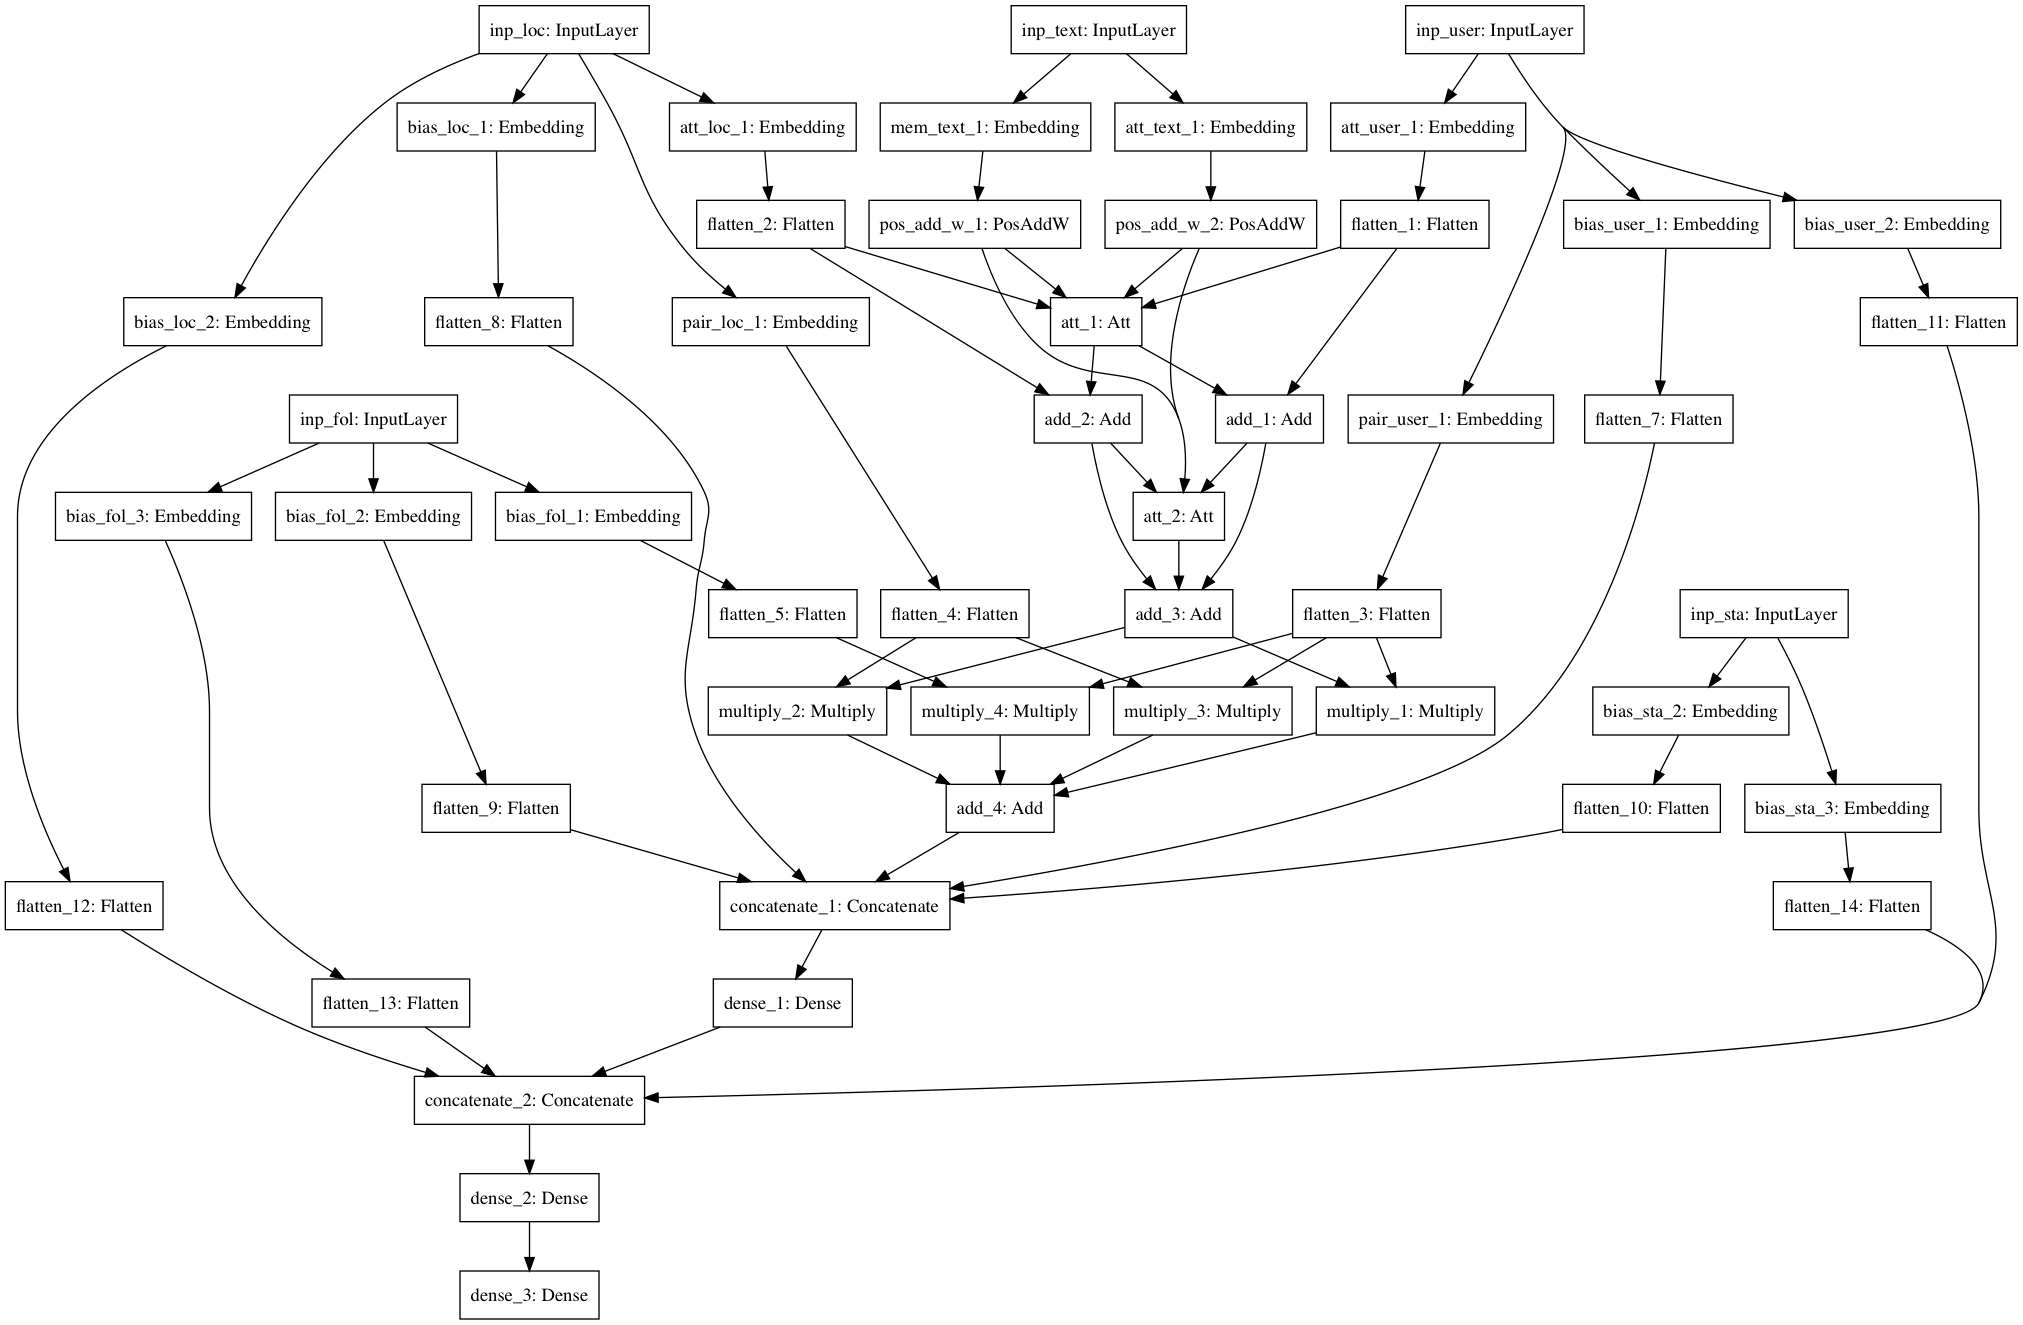
\includegraphics[width=6inc]{tweet_pics/model_noshape}

\section{实验过程}
因为网络中的层数,隐层节点数,嵌入维度等都是一个个超参数,而这些超参对模型性能有一定的影响,所以在这里我们简要的记录我们的实验过程。

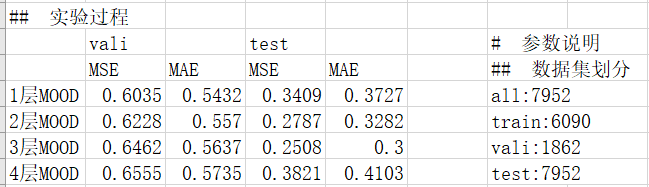
\includegraphics[width=6inc]{tweet_pics/tb}

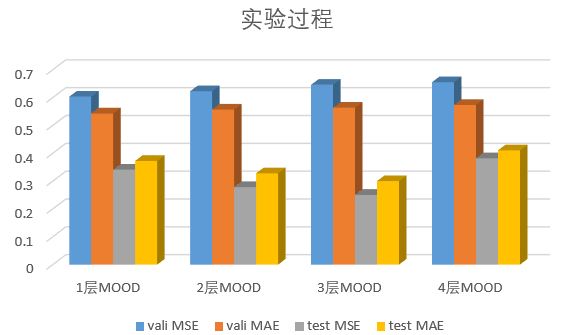
\includegraphics[width=6inc]{tweet_pics/graph}
% ———————
\renewcommand{\refname}{Reference}
\begin{thebibliography}{9}
%    \bibitem{ref-1} 专利CN105574003A
%    \bibitem{red-2} Hidden Factors and Hidden Topics: Understanding Rating Dimensions with Review Text
    \end{thebibliography}

\end{document}
